\section{Fundamental results from Fourier analysis} \label{app::Fourier}
In this appendix, we state several fundamental results from Fourier analysis for doubly periodic functions, associated with the Fourier transform pair defined in Definition~\ref{Def::Fourier}. These results are useful for us, and their proofs are well established and can be referenced in classical literature, such as in the work of Stein and Shakarchi~\cite{stein2011fourier}.
\begin{lem}\label{lem::Convolution}
	(Convolution theorem) Let $f(\bm{\rho},z)$ and $g(\bm{\rho},z)$ be two functions which are periodic in $\bm{\rho}$ and non-periodic in $z$. Suppose that $f$ and $g$ have Fourier transform $\widetilde{f}$ and $\widetilde{g}$, respectively. Their convolution is defined by
	\begin{equation}\label{eq:Q2D_cov}
		u(\bm{\rho},z):=(f\ast g)(\bm{\rho},z)=\int_{\mathcal{R}^2}\int_{\mathbb{R}}f(\bm{\rho}-\bm{\rho}',z-z')g(\bm{\rho}',z')dz'd\bm{\rho}',
	\end{equation}
	satisfying
	\begin{equation}
		\widetilde{u}(\bm{k},\kappa)=\widetilde{f}(\bm{k},\kappa)\widetilde{g}(\bm{k},\kappa).
	\end{equation}
	
\end{lem}
\begin{lem}\label{lem::Poisson}
	(Poisson summation formula) Let $f(\bm{\rho},z)$ be a function which is periodic in $\bm{\rho}$ and non-periodic in $z$. Suppose that $f$ has Fourier transform $\widetilde{f}$ and $\bm{r}=(\bm{\rho},z)$. Then one has
	\begin{equation}
		\sum_{\bm{m}\in \mathbb{Z}^2} f(\bm{r} + \V{\mathcal{M}}) = \frac{1}{2\pi L_x L_y}\sum_{\bm{k}\in \mathcal{K}^2}\int_{\mathbb{R}}\widetilde{f}(\bm{k},\kappa)e^{\m{i} \bm{k}\cdot\bm{\rho}}e^{\m{i} \kappa z}d\kappa.
	\end{equation}
\end{lem}
\begin{lem}\label{lem::2dfourier}
	(Radially symmetric functions) 
	Suppose that $f(\rho,z)$ is periodic and radially symmetric in $\bm{\rho}$, i.e., $f(\bm{\rho},z)=f(\rho,z)$. Then its Fourier transform $\widetilde{f}$ is also radially symmetric. Indeed, one has
	\begin{equation}
		\widetilde{f}(\rho,z)=2\pi\int_{0}^{\infty}J_0(k\rho)f(\rho,z)\rho d\rho.
	\end{equation}
\end{lem}

\section{Quadrature error of the trapezoidal rule}\label{app::trapezoidal}
We employ the method of contour integrals~\cite{Donaldson1972SINUA,trefethen2014Rev} to derive a precise estimation for the error in  {the} trapezoidal rule when discretizing Eqs.~\eqref{eq:ewald2d-intform1} and \eqref{eq::J02}. Consider the integral
\begin{equation}\label{eq::A.1}
I=\int_{-\infty}^{\infty }\frac{e^{-(a^2+t^2)}}{a^2+t^2}e^{\i b t}dt,
\end{equation}
where $a\geq 0$ and $b\in\mathbb{R}$. We approximate $I$ using a $(2M+1)$-point trapezoidal rule:
\begin{equation}
I_{M,\xi}=\xi\sum_{j=-M}^{M}\frac{e^{-a^2-(j\xi)^2}}{a^2+(j\xi)^2}e^{\i b j\xi},
\end{equation}
where $\xi>0$ is the step size, and we define the remainder as $E_{M,\xi}:=I-I_{M,\xi}$. Note that the integrand of $I$ has two simple poles at $t_{\pm}=\pm \i a$. Let $\Gamma_{\pm}$ be two positively/negatively oriented rectangular contours with vertices $(M+1/2)\xi\pm\i a^*$, $-(M+1/2)\xi\pm\i a^*$, $(M+1/2)\xi$, and $-(M+1/2)\xi$ (see Fig.~\ref{fig:Trapezoidal}). We enforce $a^*>a$ so that $\Gamma_{\pm}$ encloses both the interval $[-M \xi,M \xi]$ and the pole $t_{\pm}$. By following the approach given in~\cite{Donaldson1972SINUA} and applying Cauchy's theorem, we can derive an estimate for $E_{M,\xi}$ in the limit $M\rightarrow \infty$:
\begin{equation}
E_{M,\xi}=\int_{\Gamma_++\Gamma_-}\frac{e^{-(a^2+t^2)+\i b t}}{a^2+t^2}\varphi(t)dt-2\pi\i \text{Res}\left[\frac{e^{-(a^2+t^2)+\i b t}}{a^2+t^2}\varphi(t),\pm \i a\right],
\end{equation}
where
\begin{align}
\varphi(t)=\begin{cases}
\dfrac{1}{1-e^{2\pi\i t/\xi}},\,\quad &\text{Im}(t)<0,\\[1em]
-\dfrac{1}{1-e^{-2\pi\i t/\xi}},\,\quad&\text{Im}(t)>0,
\end{cases}
\end{align}
is related to the characteristic function of the trapezoidal rule, and $\text{Res}[f(t),t_0]$ denotes the residue of a function $f$ at a pole $t_0$. Since the contributions from the vertical sides of $\Gamma_{\pm}$ vanish in the limit $M\rightarrow \infty$ and by using residue calculus, we have
\begin{equation}\label{eq::A.5}
E_{M,\xi}=\left(\int_{-\infty+\i a^*}^{\infty+\i a^*}-\int_{-\infty-\i a^*}^{\infty-\i a^*}\right)\frac{e^{-(a^2+t^2)+\i b t}}{a^2+t^2}\varphi(t)dt+\frac{\pi}{a}\frac{e^{-ab}+e^{ab}}{1-e^{2\pi a/\xi}}.
\end{equation}
In Eq.~\eqref{eq::A.5}, the last term can be considered as the residue correction of the rule, while the remainder integral along $\text{Im}(t)=a^*$ can be estimated as
\begin{equation}
\begin{split}
\left|\int_{-\infty+\i a^*}^{\infty+\i a^*}\frac{e^{-(a^2+t^2)+\i b t}}{a^2+t^2}\varphi(t)dt\right|&\leq e^{(a^*)^2-a^2-a^*b-2\pi a^*/\xi}\int_{-\infty}^{\infty}\frac{|a^2+(t+\i a^*)^2|^{-1}e^{-t^2}}{\left|1-e^{2\pi\i t/\xi-2\pi a^*/\xi}\right|}dt\\
&\leq\frac{\sqrt{\pi}e^{(a^*)^2-a^2-a^*b-2\pi a^*/\xi}}{(a^*)^2-a^2}.
\end{split}
\end{equation}

To obtain a closed formula, it is necessary to determine the extremum of the exponent under the condition $a^*>a>0$. Since the range of $a$ is not specified, we can safely choose $a^*=\pi/\xi+b/2$ if $\pi/\xi+b/2>a$, and $a^*=\sqrt{a^2+1}$ otherwise. This choice ensures a decay rate of at least $\sim O(e^{-\text{sign}(\pi/\xi+b/2)|\pi/\xi+b/2|^2})$, where $\text{sign}(t)=1$ if $t> 0$, $\text{sign}(t)=0$ if $t=0$, and $\text{sign}(t)=-1$ otherwise. By following a similar procedure, we can derive that the integral along $\text{Im}(t)=-a^*$ in Eq.~\eqref{eq::A.5} decays with order $O(e^{-\text{sign}(\pi/\xi-b/2)|\pi/\xi-b/2|^2})$. Consequently, we can conclude that
\begin{equation}
E_{M,\xi}=\frac{\pi}{a}\frac{e^{-ab}+e^{ab}}{1-e^{2\pi a/\xi}}+E_{\text{err}},
\end{equation}
where the remainder error term can be estimated as 
\begin{equation}\label{eq::A.8}
|E_{\text{err}}|\sim O(e^{-\text{sign}(\pi/\xi-|b|/2)\left|\pi/\xi-|b|/2\right|^2}).
\end{equation}

\begin{figure}[!ht]
    \begin{center}
    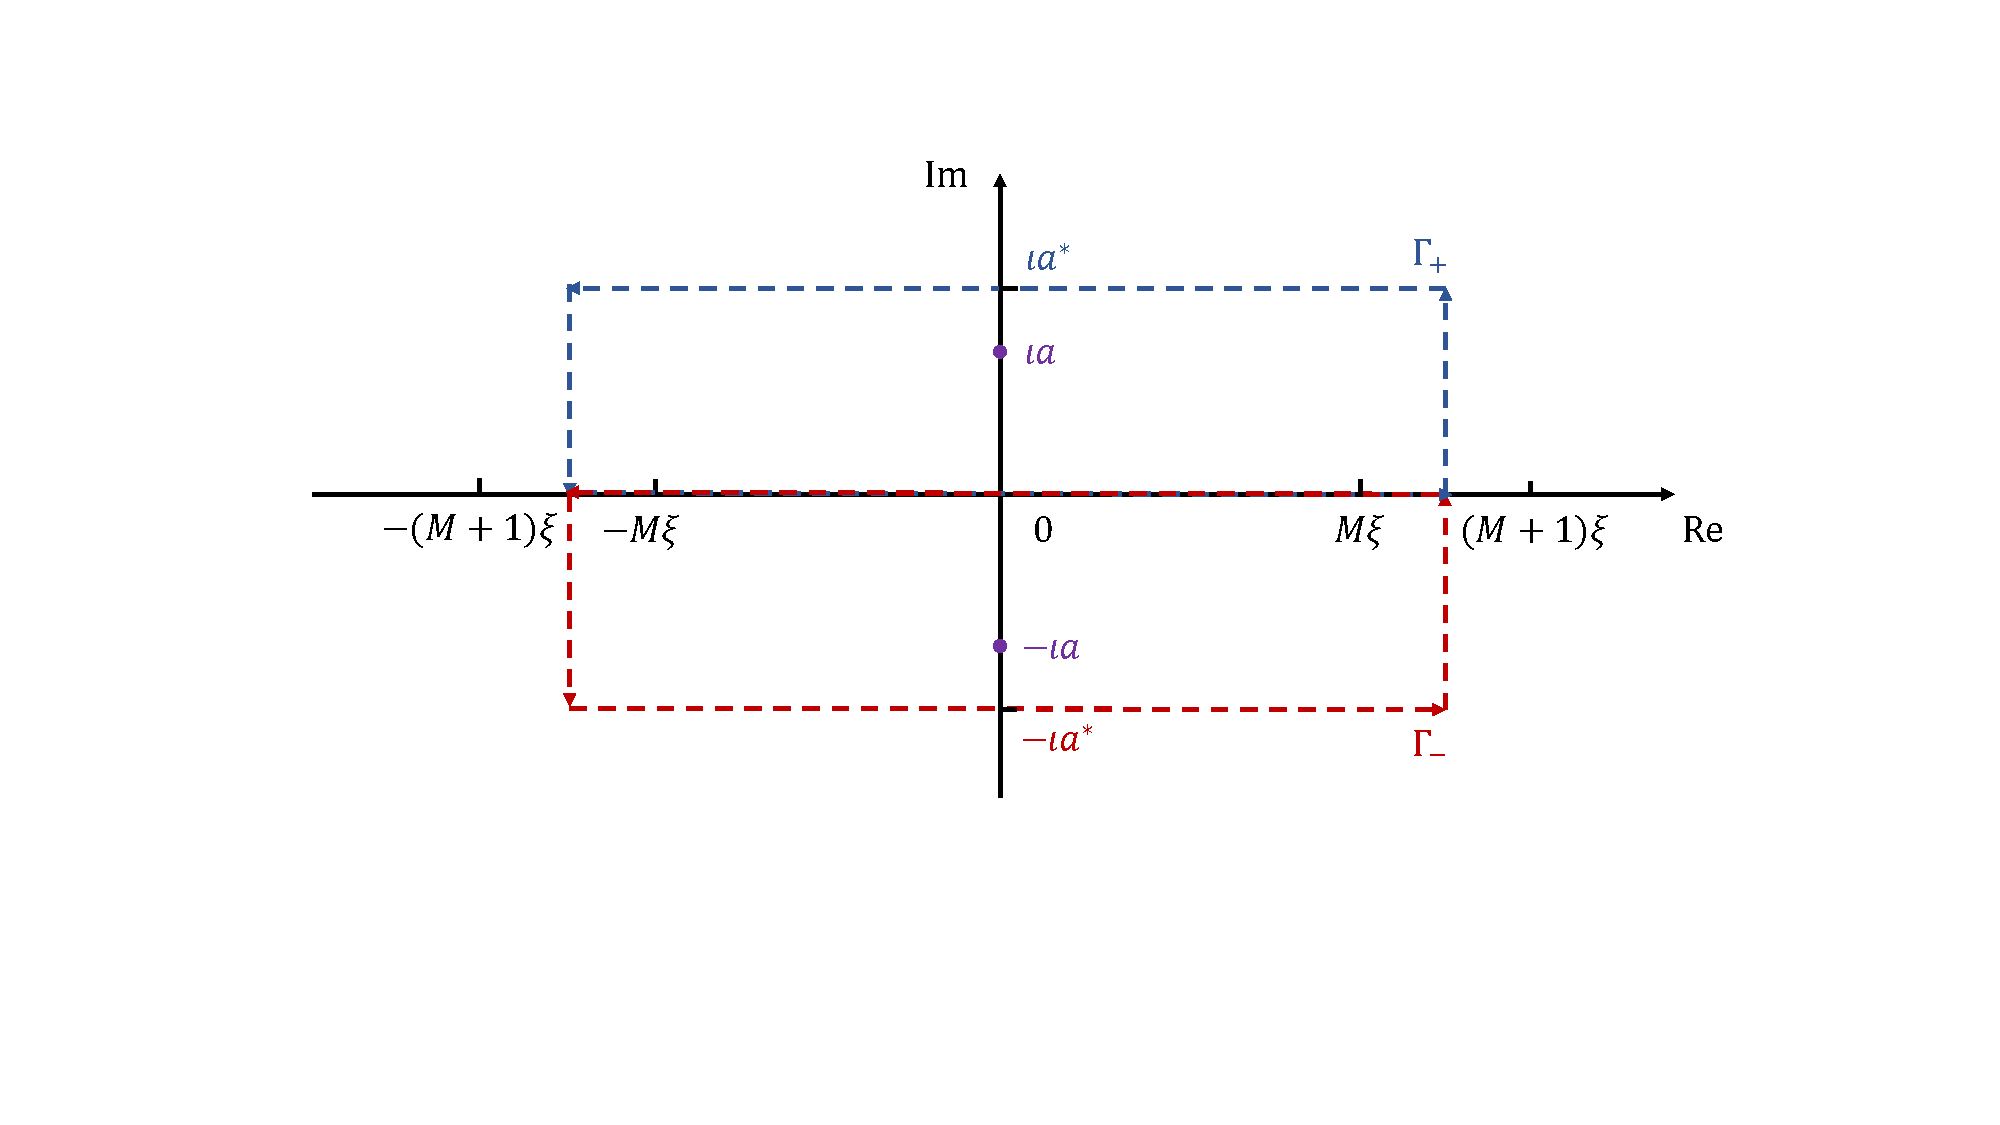
\includegraphics[width=0.8\textwidth]{figs/Trapezoidal.pdf}
    \caption{Integration contours in the error estimation of trapezoidal rule.}
    \label{fig:Trapezoidal}
    \end{center} 
\end{figure}

\section{The ideal-gas assumption}\label{app::ideal-gas}
Let $\bm{\mathcal{\psi}}$ represent a statistical quantity in an interacting particle system, and we aim to analyze its root mean square value given by
\begin{equation}\label{eq::deltaS}
    \delta \bm{\mathcal{\psi}}:=\sqrt{\frac{1}{N}\sum_{i=1}^{N}\|\bm{\mathcal{\psi}}_{i}\|^2},
\end{equation}
where $\bm{\mathcal{S}}_{i}$ denotes the quantity associated with particle $i$ (e.g., energy for one dimension or force for three dimensions). Assume that $\bm{\mathcal{\psi}}_{i}$ takes the form
\begin{equation}
	\bm{\mathcal{\psi}}_{i}=q_{i} \sum_{j \neq i} q_{j} \bm{\zeta}_{i j},
\end{equation}
due to the superposition principle of particle interactions, which implies that the total effect on particle $i$ can be expressed as the sum of contributions from each $i-j$ pair (including periodic images). Here, $\bm{\zeta}_{i j}$ represents the interaction between two particles. The ideal-gas assumption leads to the following relation
\begin{equation}
	\left\langle\boldsymbol{\zeta}_{i j} \boldsymbol{\zeta}_{i k}\right\rangle=\delta_{j k}\left\langle\boldsymbol{\zeta}_{i j}^2\right\rangle:=\delta_{j k} \zeta^2,
\end{equation}
where the expectation is taken over all particle configurations, and $\zeta$ is a constant. This assumption indicates that any two different particle pairs are uncorrelated, and the variance of each pair is expected to be uniform. In the context of computing the force variance of a charged system, this assumption implies that
\begin{equation}
	\left\langle\|\bm{\mathcal{\psi}}_{i}\|^2\right\rangle=q_{i}^2 \sum_{j, k \neq i} q_{j} q_k\left\langle\boldsymbol{\zeta}_{i j} \boldsymbol{\zeta}_{i k}\right\rangle \approx q_{i}^2 \zeta^2 Q,
\end{equation}
where $Q$ represents the total charge of the system. By applying the law of large numbers, one obtains $\delta\mathcal{\psi}\approx \zeta Q/\sqrt{N}$, which can be utilized for the mean-field estimation of the truncation error.

\section{The Debye-H$\ddot{\text{u}}$ckel approximation}\label{app::Debye}
Under the DH approximation, one is able to estimate functions associated with the $i$-th particle in the form:
\begin{equation}
	\mathscr{G}(\bm{r}_i)=\sum_{j\neq i}q_{j}e^{\m{i} \bm{k}\cdot\bm{\rho}_{ij}}f(z_{ij}),
\end{equation}
where $|f(z_{ij})|$ is bounded by a constant $C_f$ independent of $z_{ij}$. The DH theory considers the simplest model of an electrolyte solution confined to the simulation cell, where all $N$ ions are idealized as hard spheres of diameter $r_{a}$ carrying charge $\pm q$ at their centers. The charge neutrality condition requires that $N_+=N_-=N/2$. Let us fix one ion of charge $+q$ at the origin $r=0$ and consider the distribution of the other ions around it.

In the region $0<r\leq r_{a}$, the electrostatic potential $\phi(\bm{r})$ satisfies the Laplace equation $-\Delta\phi(\bm{r})=0$. For $r\geq r_{a}$, the charge density of each species is described by the Boltzmann distribution $\rho_{\pm}(\bm{r})=\pm qe^{\mp\beta q\phi(\bm{r})}\rho_r/2$ with number density $\rho_r=N/V$. In this region, the electrostatic potential satisfies the linearized Poisson-Boltzmann equation~\cite{levin2002electrostatic}:
\begin{equation}
	-\Delta \phi(\bm{r})=2\pi\left[q \rho_r e^{-\beta q\phi(\bm{r})}-q\rho_r e^{+\beta q\phi(\bm{r})}\right]\approx -4\pi \beta q^2\rho_r\phi(\bm{r}),
\end{equation}
and its solution is given by
\begin{equation}
	\phi(\bm{r})=\begin{cases}
		\dfrac{q}{4\pi r}-\dfrac{q\kappa}{4\pi (1+\kappa a)},& r<r_{a},\\[1em]
		\dfrac{qe^{\kappa a}e^{-\kappa r}}{4\pi r(1+\kappa a)},&r\geq r_{a},
	\end{cases}
\end{equation}
where $\kappa=\sqrt{\beta q^2\rho}$ denotes the inverse of Debye length $\lambda_{\text{D}}$. By this definition, the net charge density for $r>r_{a}$ is $\rho_>(\bm{r})=-\kappa^2\phi(\bm{r})$. Let us fix $\bm{r}_i$ at the origin. Given these considerations, for $r\geq r_a$, one obtains the following estimate:
\begin{equation}\label{eq::E.4}
	\begin{split}
		|\mathscr{G}(\bm{r}_i)|&\approx \left|\int_{\mathbb{R}^3\backslash B(\bm{r}_{i}, r_a)}\rho_>(\bm{r})e^{-\m{i} \bm{k}\cdot\bm{\rho}}f(z)d\bm{r}\right|\\
		&\leq \frac{q_iC_fe^{\kappa a}}{4\pi(1+\kappa a)}\int_{a}^{\infty}\frac{e^{-\kappa r}}{r}4\pi r^2dr\\
		&=q_iC_f\lambda_{\text{D}}^2.
	\end{split}
\end{equation}

It is remarked that upper bound Eq.~\eqref{eq::E.4} is derived under the continuum approximation. In the presence of surface charges, the charge distribution along the $z$-direction may lack spatial uniformity. However, due to the confinement of particle distribution between two parallel plates, the integral in Eq.~\eqref{eq::E.4} along the $z$-direction remains bounded. An upper bound in the form of $|\mathscr{G}(\bm{r}_i)|\leq C_s C_{f}q_i$ can still be expected, where $C_s$ is a constant related to the thermodynamic properties of the system.

\section{The Metropolis algorithm} \label{app::Metropolis}

In practice, the Metropolis algorithm~\cite{metropolis1953equation, hastings1970monte} is employed to generate a sequence $\{\bm{k}_{\eta}\}_{\eta=1}^{P}$ from $h(\bm{k})$. 
Since $\bm{k}\circ \bm{L}=2\pi \bm{m}$ with $\bm{m}$ an integer vector, one can conveniently sample from the discrete distribution $\mathcal{H}(\bm{m})=h(\bm{k})$ to equivalently generate $\bm{k}$. 
Once the current state of the Markov chain $\bm{m}_{\eta}=\bm{m}^{\text{old}}$ is known, the algorithm generates a random variable $\bm{m}^*$ with $m_{\xi}^*\sim \mathcal{N}[0,(\alpha L_{\xi})^2/2\pi^2]$, which is the normal distribution with mean zero and variance $(\alpha L_{\xi})^2/2\pi^2$. The new proposal is taken as $\bm{m}^{\text{new}}=\text{round}(m_{x}^*,m_{y}^*)$. To determine the acceptance rate, one obtains the proposal probability 
\begin{equation}
	q(\bm{m}^{\text{new}}|\bm{m}^{\text{old}})=\prod_{\xi\in\{x,y\}}q(m^{\text{new}}_{\xi}|m^{\text{old}}_{\xi})
\end{equation}
where
\begin{equation}
	\begin{split}
		q(m^{\text{new}}_{\xi}|m^{\text{old}}_{\xi})&=\sqrt{\frac{\pi}{(\alpha L_{\xi})^2}}\int_{m^{\text{new}}_{\xi}-\frac{1}{2}}^{m^{\text{new}}_{\xi}+\frac{1}{2}}e^{-\pi^2t^2/(\alpha L_{\xi})^2}dt\\[1em]
		&=\begin{cases}
			\erf\left(\dfrac{\pi}{2\alpha L_{\xi}}\right),&m_{\xi}^{\text{new}}=0,\\[1.15em]
			\dfrac{1}{2}\left[\erf\left(\dfrac{\pi(2|m_{\xi}^{\text{new}}|+1)}{2\alpha L_{\xi}}\right)-\erf\left(\dfrac{\pi(2|m_{\xi}^{\text{new}}|-1)}{2\alpha L_{\xi}}\right)\right],&m_{\xi}^{\text{new}}\neq 0.
		\end{cases}
	\end{split}
\end{equation}
It is worth noting that the proposal distribution $q(\bm{m}^{\text{new}}|\bm{m}^{\text{old}})$ in the Metropolis algorithm presented here does not depend on the current state $\bm{m}^{\text{old}}$. The Metropolis acceptance probability is computed using the formula:
\begin{equation}
	a(\bm{m}^{\text{new}}|\bm{m}^{\text{old}}):=\min\left\{\frac{\mathcal{H}(\bm{m}^{\text{new}})q(\bm{m}^{\text{old}}|\bm{m}^{\text{new}})}{\mathcal{H}(\bm{m}^{\text{old}})q(\bm{m}^{\text{new}}|\bm{m}^{\text{old}})},1\right\}.
\end{equation}
If the proposal is rejected, then $\bm{m}_{\eta+1}=\bm{m}_{\eta}$. If $\bm{m}^{\text{new}}$ is accepted, then $\bm{m}_{\eta+1}=\bm{m}^{\text{new}}$. The sampling procedure has a small error since $\mathcal{H}(\bm{m}^{\text{new}})\approx q(\bm{m}^{\text{new}}|\bm{m}^{\text{old}})$. Our numerical experiments show an average acceptance rate of over $90\%$. Additionally, one can set an integer downsampling rate $\mathscr{D}$, where only one sample is taken from every $\mathscr{D}$ samples, to reduce the correlation between batches in the Metropolis process.

\section{Physical quantities}\label{Sec::phyquan}

In this section, we will briefly describe how to calculate the physical quantities of interest in this paper.

To calculate the average concentration of the system along the $z$-direction, we first divide the interval $[0,H]$ into $250$ equally spaced bins. Then, every $100$ steps, we count the number of particles whose $z$-coordinate $r_z$ falls within each bin and calculate the ensemble average. After the simulation is completed, we divide the accumulated values by the length of each bin to obtain the average concentration. The MSD along $z$-direction, $\eta_{\text{msd},z}(t)$ at time $t$ is defined as
\begin{equation}
\eta_{\mathrm{msd},z}(t)=\left\langle\left|r_z\left(t+t_0\right)-r_z\left(t_0\right)\right|^2\right\rangle,
\end{equation}
with the bracket representing the ensemble average over $t_0$. The VACF along $z$-direction, $\eta_{\text{vacf},z}(t)$ at time $t$ is defined as
\begin{equation}
\eta_{\text {vacf},z}(t)=\left\langle v_z\left(t_0\right) v_z(t)\right\rangle,
\end{equation}
with the bracket representing the ensemble average over $t_0$. The total energy is defined as the sum of potential energy and kinetic energy. The potential energy is the sum of bond, angle, Coulomb, LJ and  {constraint} components, where the first two and the last one are not required for electrolyte solutions. 

Let $N$ is the number of particles, $\bm{r}_i=(r_{i,x},r_{i,y},r_{i,z})$, $\bm{v}_i=(v_{i,x},v_{i,y},v_{i,z})$ and $\bm{f}_i=(f_{i,x},f_{i,y},f_{i,z})$ represent the position, velocity and force of $i$th particle along each of three dimensions, respectively. The $z$-$z$ component subtracted from pressure tensor is computed by the formula
\begin{equation}
P_{zz}=\frac{1}{V} \sum_{i=1}^N\left(m_i v_{i,z} v_{i, z}+r_{i,z} f_{i,z}\right),
\end{equation}
where the two components in each term come from the kinetic energy and the virial contributions, respectively. It is remarked that the far-field component of  {the} virial associated with the Ewald decomposition requires the use of specialized methods~\cite{liang2022random}. 